\subsection{Machine learning based reconstruction of the hadronically decaying W boson}


This section give a more in-depth description of the machine-learning model that is introduced for the reconstruction of the hadronically decaying \Wboson boson in Section... \\
This study demonstrates that the ML-based reconstruction performs well on the bulk of events, while struggling to capture the structure of the phase space edges. The five leading light jets are considered as input. All possible 1-, 2-, and 3-jet combinations are considered.
A total of 25 jet candidates is found and their 4-vectors are passed to the network as input.
A classification network is trained. The candidate which minimizes $\Delta R(\Wtruth, \Wcand)$ is labeled with "1", while all other candidates are assigned the label "0".

The candidate features are processed through a sequence of five dense layers with ReLU activation functions.
The architecture consists of 8,16,32,16,8 nodes, respectively.
A dropout layer with a dropout rate of $20\%$ is added after the second and third layer to reduce the risk of overfitting during the training step.
The 25 output nodes are normalized vy applying a softmax activation function, such that the output score can be interpreted as a probability.
The Adam optimizer with categorical cross-entropy is used as loss function.


\begin{figure}[ht!]
	\centering
	\begin{subfigure}[b]{0.49\linewidth}
		\includegraphics[width=1.\linewidth, page=3]{figures/WbWb/WhadReconstruction/part_ml_study.pdf}
		\caption{Loss curve for particle level.}
		\label{fig:WhadrecoML:loss_part}
	\end{subfigure}
	\begin{subfigure}[b]{0.49\linewidth}
		\includegraphics[width=1.\linewidth, page=3]{figures/WbWb/WhadReconstruction/reco_ml_study.pdf}
		\caption{Loss curve for detector level NN.}
		\label{fig:WhadrecoML:loss_reco}
	\end{subfigure}
	\caption{Loss function minimized during the training of the neural network. Separate networks are trained for the particle and detector level reconstruction. The loss curve is shown for the training as well as for the validation set.}
	\label{fig:Whadreco:loss}
\end{figure}

Separate networks are trained for the particle and detector level reconstruction.
The loss curves which are obtained for every single training epoch are displayed in Figure~\ref{fig:WhadrecoML:loss}.
The fraction of events used for validation is $20\%$.

After a steep decline, the loss is flattening out. 
Similar values are obtained for training and validation set, indicating no over-fitting of the model
Early stopping / values from best iteration used.


\begin{figure}[ht!]
	\centering
	\begin{subfigure}[b]{0.42\linewidth}
		\includegraphics[width=\linewidth, page=7]{figures/WbWb/WhadReconstruction/part_ml_study.pdf}
		\caption{Transverse momentum.}
		\label{fig:WhadrecoML:reso_pt_part}
	\end{subfigure}
	\begin{subfigure}[b]{0.42\linewidth}
		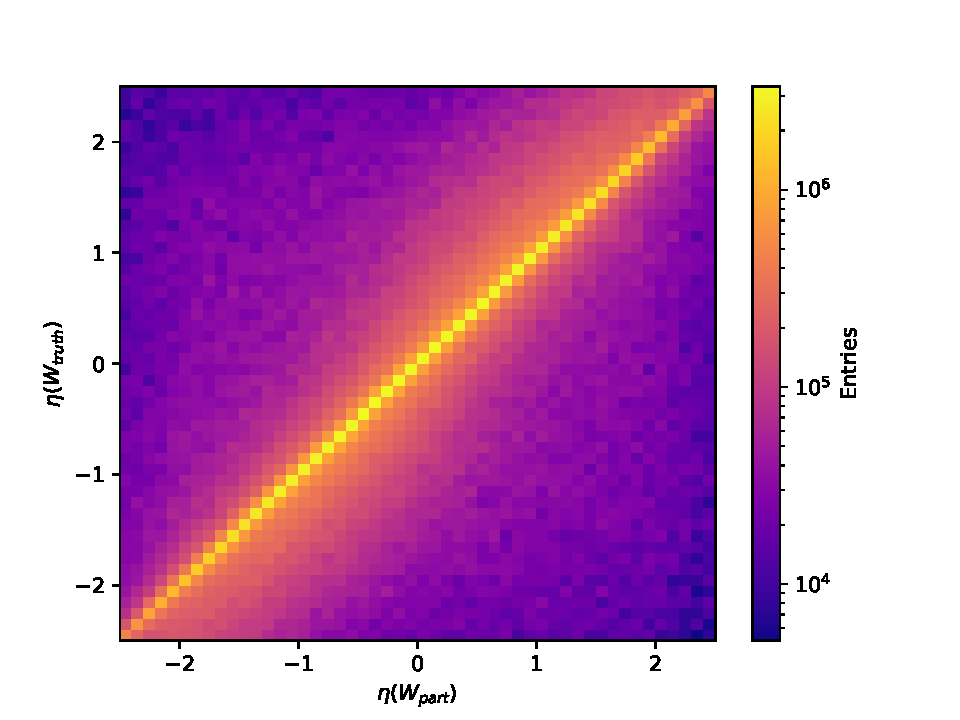
\includegraphics[width=\linewidth, page=1]{figures/WbWb/WhadReconstruction/part_ml_study.pdf}
		\caption{Pseudo-rapidity.}
		\label{fig:WhadrecoML:reso_eta_part}
	\end{subfigure}
	\\
	\begin{subfigure}[b]{0.42\linewidth}
		\includegraphics[width=\linewidth, page=4]{figures/WbWb/WhadReconstruction/part_ml_study.pdf}
		\caption{Azimuthal angle.}
		\label{fig:WhadrecoML:reso_phi_part}
	\end{subfigure}
	\caption{Resolution plots for the ML-based \Whad particle level reconstruction. The kinematic observables transverse momentum \pT (\ref{fig:WhadrecoML:reso_pt_part}), pseudo-rapidity $\eta$ (\ref{fig:WhadrecoML:reso_eta_part}) and azimuthal angle $\varphi$ (\ref{fig:WhadrecoML:reso_phi_part}) of the particle level \Whad candidate are being compared to \Wtruth.}
	\label{fig:WhadrecoML:resolution_part}
\end{figure}

\begin{figure}[ht!]
	\centering
	\begin{subfigure}[b]{0.42\linewidth}
		\includegraphics[width=\linewidth, page=7]{figures/WbWb/WhadReconstruction/reco_ml_study.pdf}
		\caption{Transverse momentum.}
		\label{fig:WhadrecoML:reso_pt_reco}
	\end{subfigure}
	\begin{subfigure}[b]{0.42\linewidth}
		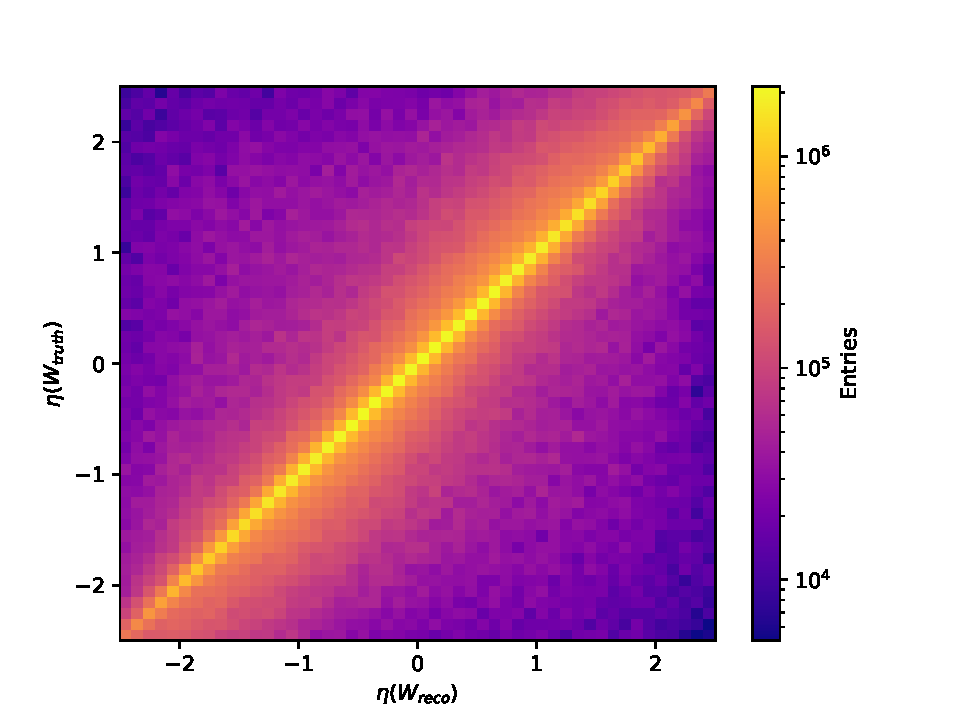
\includegraphics[width=\linewidth, page=1]{figures/WbWb/WhadReconstruction/reco_ml_study.pdf}
		\caption{Pseudo-rapidity.}
		\label{fig:WhadrecoML:reso_eta_reco}
	\end{subfigure}
	\\
	\begin{subfigure}[b]{0.42\linewidth}
		\includegraphics[width=\linewidth, page=4]{figures/WbWb/WhadReconstruction/reco_ml_study.pdf}
		\caption{Azimuthal angle.}
		\label{fig:WhadrecoML:reso_phi_reco}
	\end{subfigure}
	\caption{Resolution plots for the ML-based \Whad reconstruction on detector level. The kinematic observables transverse momentum \pT (\ref{fig:WhadrecoML:reso_pt_reco}), pseudo-rapidity $\eta$ (\ref{fig:WhadrecoML:reso_pt_reco}) and azimuthal angle $\varphi$ (\ref{fig:WhadrecoML:reso_phi_reco}) of the \Whad candidate are being compared to \Wtruth.}
	\label{fig:WhadrecoML:resolution_reco}
\end{figure}

Figure~\ref{fig:WhadrecoML:resolution_part} compares the particle level candidate identified by the NN to \Wtruth with respect to their kinematic properties.
The resolution plots are dominated by the diagonal elements, with improving performance towards higher momenta.
Similar results are obtained for the detector level reconstruction in Figure~\ref{fig:WhadrecoML:resolution_reco}.
The broadening of the diagonal elements is a direct consequence of the imperfect detector resolution.


\begin{figure}[ht!]
	\centering
	\begin{subfigure}[b]{1.0\linewidth}
		\includegraphics[width=1.\linewidth, page=10]{figures/WbWb/WhadReconstruction/part_ml_study.pdf}
		%\caption{Transverse momentum.}
		\label{fig:WhadrecoML:score_00_03_part}
	\end{subfigure}
	\begin{subfigure}[b]{1.0\linewidth}
		\includegraphics[width=1.\linewidth, page=8]{figures/WbWb/WhadReconstruction/part_ml_study.pdf}
		%\caption{Pseudo-rapidity.}
		\label{fig:WhadrecoML:score_03_07_part}
	\end{subfigure}
	\begin{subfigure}[b]{1.0\linewidth}
		\includegraphics[width=1.\linewidth, page=9]{figures/WbWb/WhadReconstruction/part_ml_study.pdf}
		%\caption{Azimuthal angle.}
		\label{fig:WhadrecoML:score_07_10_part}
	\end{subfigure}
	\caption{Loss function minimized during the training of the neural network. Separate networks are trained for the particle and detector level reconstruction. The loss curve is shown for the training as well as for the validation set.}
	\label{fig:WhadrecoML:score_part}
\end{figure}

\begin{figure}[ht!]
	\centering
	\begin{subfigure}[b]{1.0\linewidth}
		\includegraphics[width=1.\linewidth, page=10]{figures/WbWb/WhadReconstruction/reco_ml_study.pdf}
		%\caption{Transverse momentum.}
		\label{fig:WhadrecoML:score_00_03_reco}
	\end{subfigure}
	\begin{subfigure}[b]{1.0\linewidth}
		\includegraphics[width=1.\linewidth, page=8]{figures/WbWb/WhadReconstruction/reco_ml_study.pdf}
		%\caption{Pseudo-rapidity.}
		\label{fig:WhadrecoML:score_03_07_reco}
	\end{subfigure}
	\begin{subfigure}[b]{1.0\linewidth}
		\includegraphics[width=1.\linewidth, page=9]{figures/WbWb/WhadReconstruction/reco_ml_study.pdf}
		%\caption{Azimuthal angle.}
		\label{fig:WhadrecoML:score_07_10_reco}
	\end{subfigure}
	\caption{Loss function minimized during the training of the neural network. Separate networks are trained for the particle and detector level reconstruction. The loss curve is shown for the training as well as for the validation set.}
	\label{fig:WhadrecoML:score_reco}
\end{figure}

Figures~\ref{fig:WhadrecoML:score_part} and~\ref{fig:WhadrecoML:score_reco} show the index, \Wcand mass and light jet multiplicity distributions for particle and detector level, respectively.




Resolution plots are shown comparing reco and truth level for the W reco with and without mass cut
\begin{figure}[ht!]
	\centering
	\begin{subfigure}[b]{0.3\linewidth}
		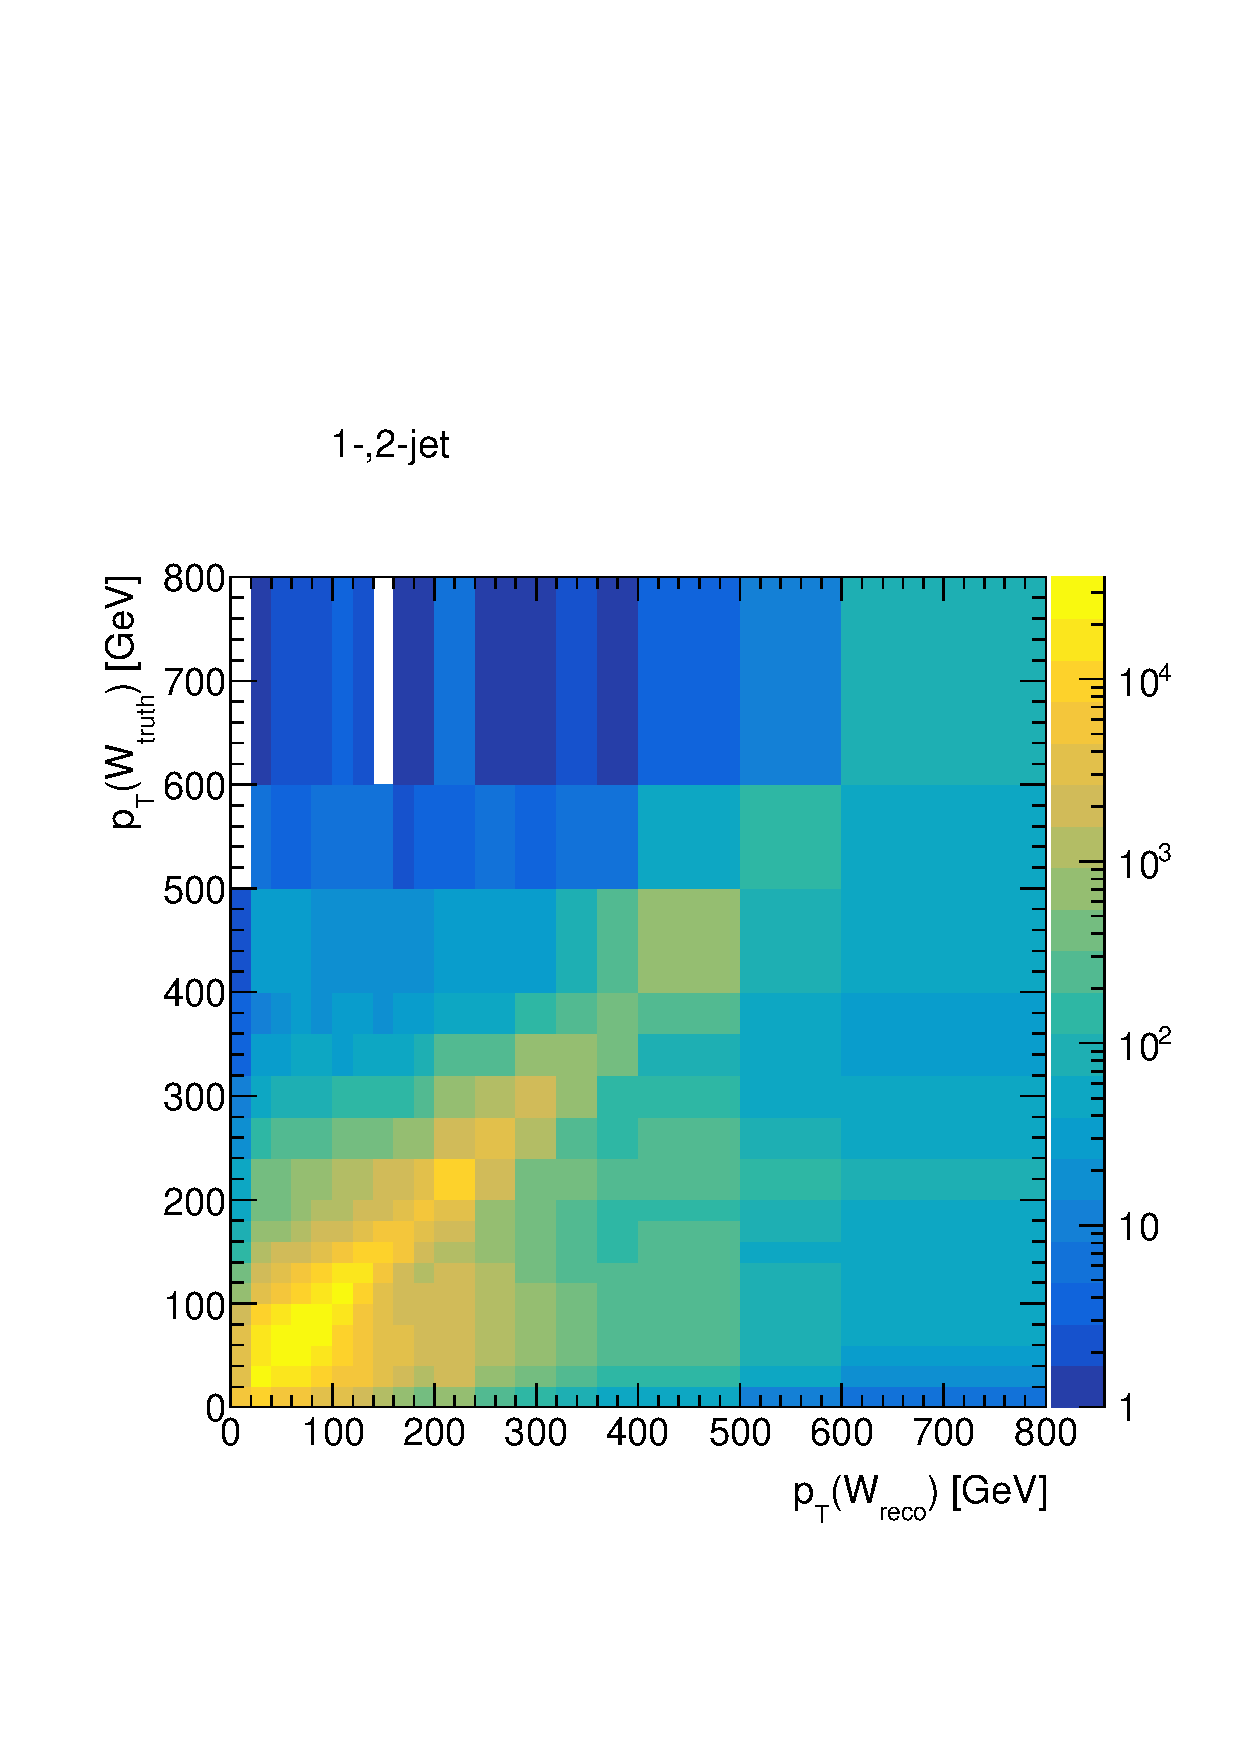
\includegraphics[trim={1cm 3cm 1cm 8cm},clip, width=1.\linewidth, page=1]{figures/WbWb/WhadReconstruction/resolution_j12_three_pt_ordered.pdf}
		%\caption{\pT resolution.}
		\label{fig:Whadreco:resolution_pt}
	\end{subfigure}
	\begin{subfigure}[b]{0.3\linewidth}
		\includegraphics[trim={1cm 3cm 1cm 8cm},clip, width=1.\linewidth, page=2]{figures/WbWb/WhadReconstruction/resolution_j12_three_pt_ordered.pdf}
		%\caption{\pT resolution with mass cut.}
		\label{fig:Whadreco:resolution_pt_masscut}
	\end{subfigure}
	\\
	\begin{subfigure}[b]{0.3\linewidth}
		\includegraphics[trim={1cm 3cm 1cm 8cm},clip, width=1.\linewidth, page=3]{figures/WbWb/WhadReconstruction/resolution_j12_three_pt_ordered.pdf}
		%\caption{Rapidity resolution.}
		\label{fig:Whadreco:resolution_y}
	\end{subfigure}
	\begin{subfigure}[b]{0.3\linewidth}
		\includegraphics[trim={1cm 3cm 1cm 8cm},clip, width=1.\linewidth, page=4]{figures/WbWb/WhadReconstruction/resolution_j12_three_pt_ordered.pdf}
		%\caption{Rapidity resolution with mass cut.}
		\label{fig:Whadreco:resolution_y_masscut}
	\end{subfigure}
	\\
	\begin{subfigure}[b]{0.3\linewidth}
	\includegraphics[trim={1cm 3cm 1cm 8cm},clip, width=1.\linewidth, page=5]{figures/WbWb/WhadReconstruction/resolution_j12_three_pt_ordered.pdf}
	%\caption{\pT resolution.}
	\label{fig:Whadreco:resolution_eta}
	\end{subfigure}
	\begin{subfigure}[b]{0.3\linewidth}
		\includegraphics[trim={1cm 3cm 1cm 8cm},clip, width=1.\linewidth, page=6]{figures/WbWb/WhadReconstruction/resolution_j12_three_pt_ordered.pdf}
		%\caption{\pT resolution with mass cut.}
			\label{fig:Whadreco:resolution_eta_masscut}
	\end{subfigure}
	\\
	\begin{subfigure}[b]{0.3\linewidth}
		\includegraphics[trim={1cm 3cm 1cm 8cm},clip, width=1.\linewidth, page=7]{figures/WbWb/WhadReconstruction/resolution_j12_three_pt_ordered.pdf}
		%\caption{Rapidity resolution.}
		\label{fig:Whadreco:resolution_m}
	\end{subfigure}
	\begin{subfigure}[b]{0.3\linewidth}
		\includegraphics[trim={1cm 3cm 1cm 8cm},clip, width=1.\linewidth, page=8]{figures/WbWb/WhadReconstruction/resolution_j12_three_pt_ordered.pdf}
		%\caption{Rapidity resolution with mass cut.}
		\label{fig:Whadreco:resolution_m_masscut}
	\end{subfigure}
		\caption{Add caption.}
		\label{fig:Whadreco:resolution}
\end{figure}
	
\begin{figure}[ht!]
	\centering
	\begin{subfigure}[b]{0.3\linewidth}
		\includegraphics[trim={1cm 3cm 1cm 8cm},clip, width=1.\linewidth, page=17]{figures/WbWb/WhadReconstruction/resolution_j12_three_pt_ordered.pdf}
		%\caption{\pT resolution.}
		\label{fig:Whadpart:resolution_pt}
	\end{subfigure}
	\begin{subfigure}[b]{0.3\linewidth}
		\includegraphics[trim={1cm 3cm 1cm 8cm},clip, width=1.\linewidth, page=18]{figures/WbWb/WhadReconstruction/resolution_j12_three_pt_ordered.pdf}
		%\caption{\pT resolution with mass cut.}
		\label{fig:Whadpart:resolution_pt_masscut}
	\end{subfigure}
	\\
	\begin{subfigure}[b]{0.3\linewidth}
		\includegraphics[trim={1cm 3cm 1cm 8cm},clip, width=1.\linewidth, page=19]{figures/WbWb/WhadReconstruction/resolution_j12_three_pt_ordered.pdf}
		%\caption{Rapidity resolution.}
		\label{fig:Whadpart:resolution_y}
	\end{subfigure}
	\begin{subfigure}[b]{0.3\linewidth}
		\includegraphics[trim={1cm 3cm 1cm 8cm},clip, width=1.\linewidth, page=20]{figures/WbWb/WhadReconstruction/resolution_j12_three_pt_ordered.pdf}
		%\caption{Rapidity resolution with mass cut.}
		\label{fig:Whadpart:resolution_y_masscut}
	\end{subfigure}
	\\
	\begin{subfigure}[b]{0.3\linewidth}
		\includegraphics[trim={1cm 3cm 1cm 8cm},clip, width=1.\linewidth, page=21]{figures/WbWb/WhadReconstruction/resolution_j12_three_pt_ordered.pdf}
		%\caption{\pT resolution.}
		\label{fig:Whadpart:resolution_eta}
	\end{subfigure}
	\begin{subfigure}[b]{0.3\linewidth}
		\includegraphics[trim={1cm 3cm 1cm 8cm},clip, width=1.\linewidth, page=22]{figures/WbWb/WhadReconstruction/resolution_j12_three_pt_ordered.pdf}
		%\caption{\pT resolution with mass cut.}
		\label{fig:Whadpart:resolution_eta_masscut}
	\end{subfigure}
	\\
	\begin{subfigure}[b]{0.3\linewidth}
		\includegraphics[trim={1cm 3cm 1cm 8cm},clip, width=1.\linewidth, page=23]{figures/WbWb/WhadReconstruction/resolution_j12_three_pt_ordered.pdf}
		%\caption{Rapidity resolution.}
		\label{fig:Whadpart:resolution_m}
	\end{subfigure}
	\begin{subfigure}[b]{0.3\linewidth}
		\includegraphics[trim={1cm 3cm 1cm 8cm},clip, width=1.\linewidth, page=24]{figures/WbWb/WhadReconstruction/resolution_j12_three_pt_ordered.pdf}
		%\caption{Rapidity resolution with mass cut.}
		\label{fig:Whadpart:resolution_m_masscut}
	\end{subfigure}
	\caption{Add caption.}
	\label{fig:Whadpart:resolution}
\end{figure}
